\documentclass[a4paper,12pt]{book}

% Paquetes necesarios
\usepackage[utf8]{inputenc}   % Codificación de caracteres
\usepackage[spanish]{babel}   % Idioma español
\usepackage[T1]{fontenc}      % Codificación de fuentes
\usepackage{amsmath, amssymb} % Símbolos matemáticos
\usepackage{graphicx}         % Inclusión de gráficos
\usepackage{cite}             % Gestión de citas
\usepackage{hyperref}         % Enlaces y referencias
\usepackage{geometry}         % Configuración de márgenes
\usepackage{fancyhdr}         % Encabezados y pies de página
\usepackage{titlesec}         % Formato de títulos
\usepackage{booktabs}         % Tablas profesionales
\usepackage{caption}          % Personalización de leyendas
\usepackage{enumitem}         % Personalización de listas
\usepackage{float}
\usepackage{tcolorbox}
\usepackage[table]{xcolor} % Paquete para colores en tablas
\usepackage{colortbl}       % Complemento para colorear celdas específicas
\usepackage{multirow}       % Combinar celdas en tablas
\usepackage{makecell}       % Combinar celdas en tablas
\usepackage{enumitem}
\usepackage{amsmath}
\usepackage{eurosym}
\usepackage{tikz}
\usepackage{listings}
\usepackage{color}
\usepackage{float}
\usepackage{pdfpages}
\usepackage{subcaption}
\usepackage{pgffor}
\usepackage{stackengine}
\usetikzlibrary{shapes, arrows, positioning}
% Configuración de márgenes
\geometry{left=3cm, right=3cm, top=2.5cm, bottom=2.5cm}
\usetikzlibrary{calc}


% Configuración de encabezados y pies de página
% \setlength{\headheight}{14.49998pt}
\pagestyle{fancy}
\fancyhf{}
\fancyhead[L]{Universidad de Granada}
\fancyhead[L]{\nouppercase{\leftmark}}

% \fancyhead[C]{Escuela Técnica Superior de Ingenierías Informática}
\fancyhead[R]{Fundamentos de Base de Datos}
\fancyfoot[L]{\rule[0pt]{\textwidth}{0.2pt}\\Ismael Sallami Moreno}
\fancyfoot[C]{\rule[0pt]{\textwidth}{0.2pt}\\\thepage}
\fancyfoot[R]{\rule[0pt]{\textwidth}{0.2pt}\\\today}
\renewcommand{\sectionmark}[1]{\markboth{#1}{}} % Configura \leftmark para que solo muestre la sección

% \renewcommand{\ejercicio}[1]{%
%     \ifnum#1=8
%         Ejercicio 1. Primera forma.%%
%     \else\ifnum#1=9
%         Ejercicio 1. Segunda forma.%%
%     \else\ifnum#1=10
%         Ejercicio 2.%
%     \else\ifnum#1=11
%         Ejercicio 3.%
%     \else\ifnum#1=12
%         Ejercicio 4.%
%     \else\ifnum#1=13
%         Ejercicio 5. Primera forma.%
%     \else\ifnum#1=14
%         Ejercicio 5. Segunda forma.%
%     \else\ifnum#1=15
%         Ejercicio 6. Primera forma.%
%     \else\ifnum#1=16
%         Ejercicio 6. Segunda forma.%
%     \else\ifnum#1=17
%         Ejercicio 7.%
%     \else\ifnum#1=18
%         Ejercicio 8.%
%     \else\ifnum#1=19
%         Ejercicio 9.%
%     \else\ifnum#1=20
%         Ejercicio 10.%
%     \else\ifnum#1=21
%         Ejercicio 11.%
%     \else\ifnum#1=22
%         Ejercicio 12.%
%     \else\ifnum#1=23
%         Ejercicio 13.%
%     \else\ifnum#1=24
%         Ejercicio 14.%
%     \else\ifnum#1=25
%         Ejercicio 15.%
%     \else\ifnum#1=26
%         Ejercicio 16.%
%     \else
%         Ejercicio #1%
%     \fi\fi\fi\fi\fi\fi\fi\fi\fi\fi\fi\fi\fi\fi\fi\fi\fi\fi\fi\fi\fi\fi\fi\fi\fi\fi
% }

\newcommand{\ejercicio}[1]{%
    \ifcase#1
        % No hay caso 0
    \or % Caso 1
        % No hay caso 1
    \or % Caso 2
        % No hay caso 2
    \or % Caso 3
        % No hay caso 3
    \or % Caso 4
        % No hay caso 4
    \or % Caso 5
        % No hay caso 5
    \or % Caso 6
        % No hay caso 6
    \or % Caso 7
        % No hay caso 7
    \or % Caso 8
        Ejercicio 1. Primera forma. Formato libreta.
    \or % Caso 9
        Ejercicio 1. Segunda forma. Formato libreta.
    \or % Caso 10
        Ejercicio 2. Formato libreta.
    \or % Caso 11
        Ejercicio 3. Formato libreta.
    \or % Caso 12
        Ejercicio 4. Formato libreta.
    \or % Caso 13
        Ejercicio 5. Primera forma. Formato libreta.
    \or % Caso 14
        Ejercicio 5. Segunda forma. Formato libreta.
    \or % Caso 15
        Ejercicio 6. Primera forma. Formato libreta.
    \or % Caso 16
        Ejercicio 6. Segunda forma. Formato libreta.
    \or % Caso 17
        Ejercicio 7. Formato libreta.
    \or % Caso 18
        Ejercicio 8. Formato libreta.
    \or % Caso 19
        Ejercicio 9. Formato libreta.
    \or % Caso 20
        Ejercicio 10. Formato libreta.
    \or % Caso 21
        Ejercicio 11. Formato libreta.
    \or % Caso 22
        Ejercicio 12. Formato libreta.
    \or % Caso 23
        Ejercicio 13. Formato libreta.
    \or % Caso 24
        Ejercicio 14. Formato libreta.
    \or % Caso 25
        Ejercicio 15. Formato libreta.
    \or % Caso 26
        Ejercicio 16. Formato libreta.
    \else
        Ejercicio #1. Formato libreta.
    \fi
}




% Formato de títulos
\titleformat{\section}{\large\bfseries}{\thesection.}{0.5em}{}
\titleformat{\subsection}{\normalsize\bfseries}{\thesubsection.}{0.5em}{}

% Datos del documento
\title{\textbf{Temario Inteligencia Artificial}}
\author{
    Ismael Sallami Moreno \\
    \texttt{ism350zsallami@correo.ugr.es}
}
\date{
    \vspace{1cm}
    \begin{tabular}{rl}
        \textbf{Asignatura:} & Fundamentos de Base de Datos \\
        \textbf{Tema:} & Teoría \\
        \textbf{Fecha:} & \today
    \end{tabular}
}
\renewcommand{\b}[1]{\textbf{#1}}

\begin{document}

% Portada
\begin{titlepage}
    \begin{center}
        % \vspace*{1cm}
        
        % \Huge
        % \textbf{Práctica Contabilidad Financiera II}
        \Huge \textbf{Prácticas Fundamentos de Bases de Datos} 
        % \vspace{0.5cm}
        % \LARGE
        % \textbf{Ismael Sallami Moreno}\\
        % \LARGE
        % \texttt{ism350zsallami@correo.ugr.es}
        % \LARGE
        % \url{https://github.com/Ismael-Sallami}
        
        % \vfill
        
        % \Large
        % \textbf{Universidad de Granada}
        
        \vspace{0.8cm}
        
        \begin{tikzpicture}[remember picture, overlay]
            \node[opacity=0.2] at (current page.center) {
\includegraphics[width=\paperwidth,height=\paperheight]{portada.jpg}};
            \node[align=center] at (current page.center) {
                
                \vspace{0.5cm}
                \LARGE \textbf{Ismael Sallami Moreno} \\
                \LARGE \texttt{ism350zsallami@correo.ugr.es} \\
                \LARGE \url{https://ismael-sallami.github.io/} \\
                \LARGE \url{https://elblogdeismael.github.io/} \\
                \vspace{2cm}
                \Large \textbf{Universidad de Granada} \\
                \vspace{0.8cm}
                % \Large \textbf{2025}
            };
        \end{tikzpicture}
        \vfill
        
        \Large
        \textbf{2025}
        
    \end{center}
\end{titlepage}
\newpage


%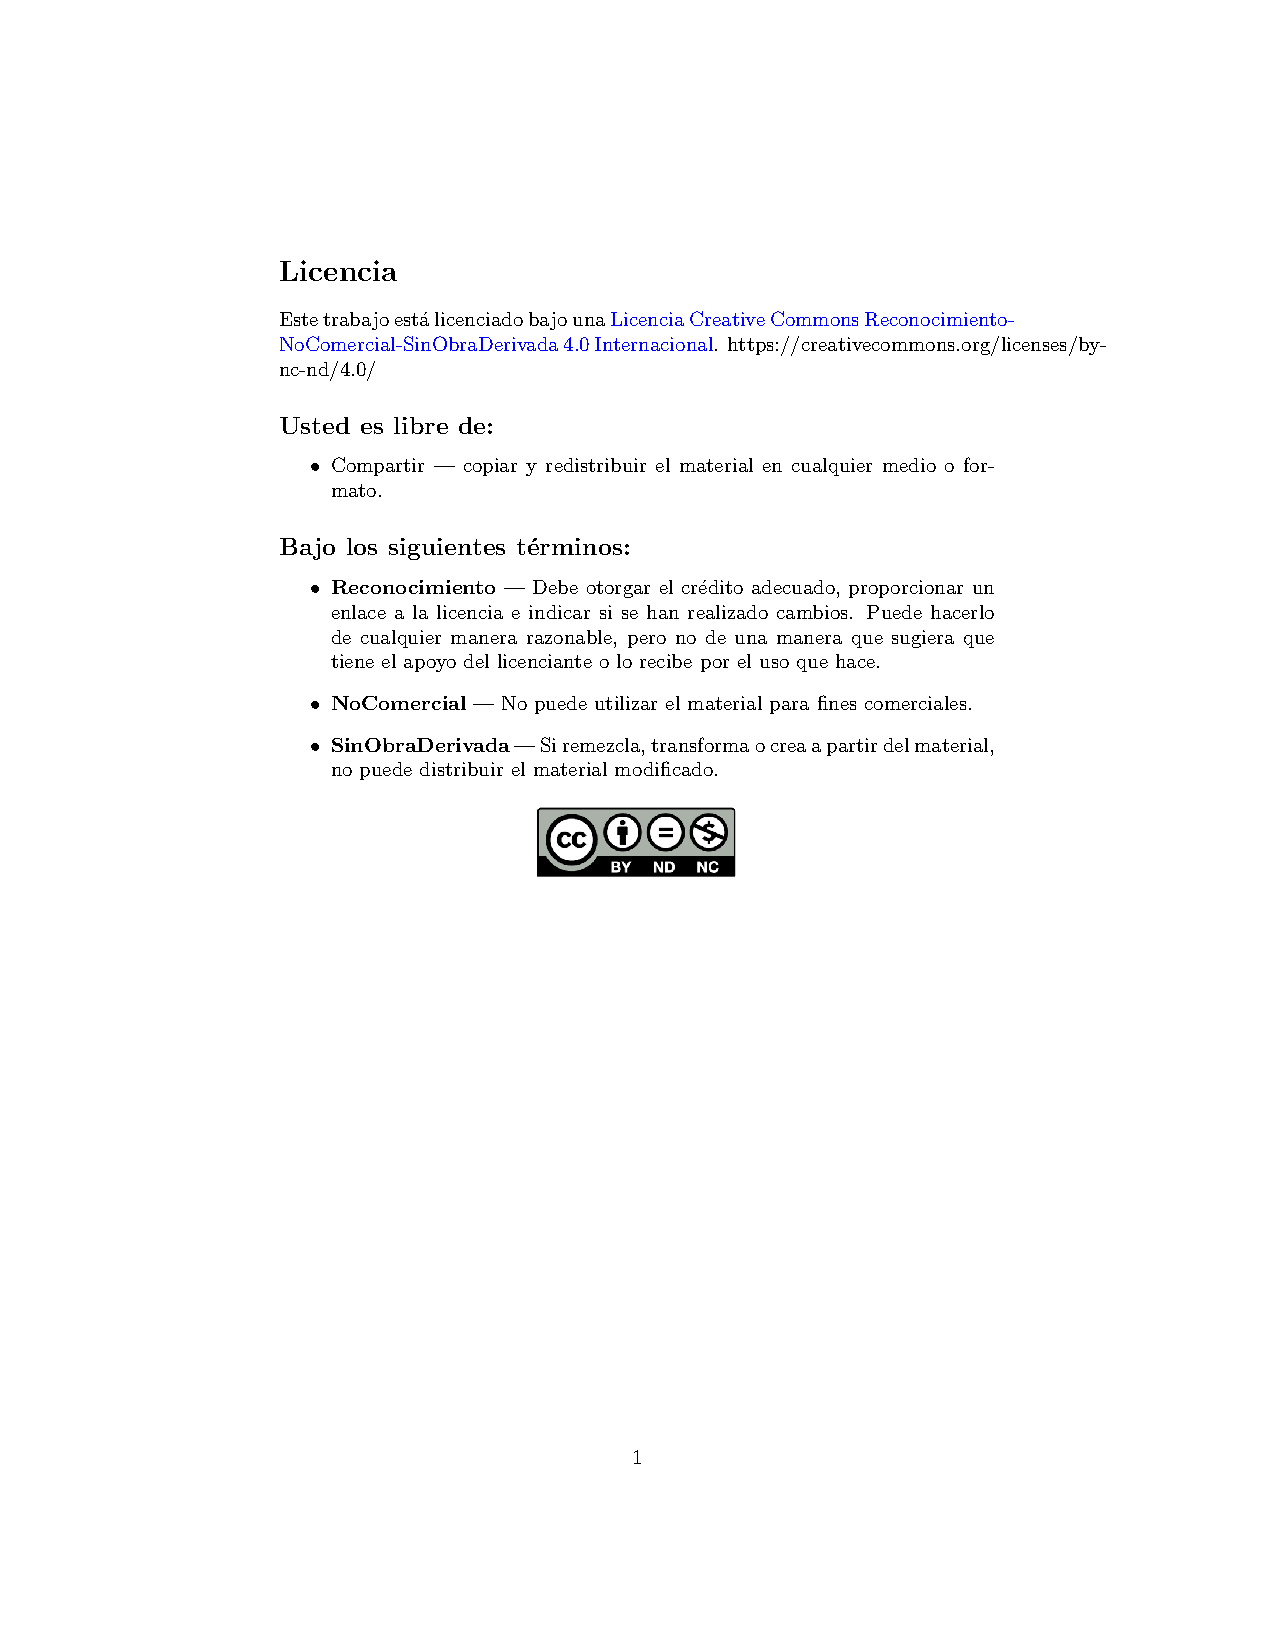
\includepdf[pages=-]{../../../../licencia.pdf}

% Tabla de contenidos
\tableofcontents
\newpage
\chapter{Modelado Conceptual}
\section{Relación de Ejercicios}
%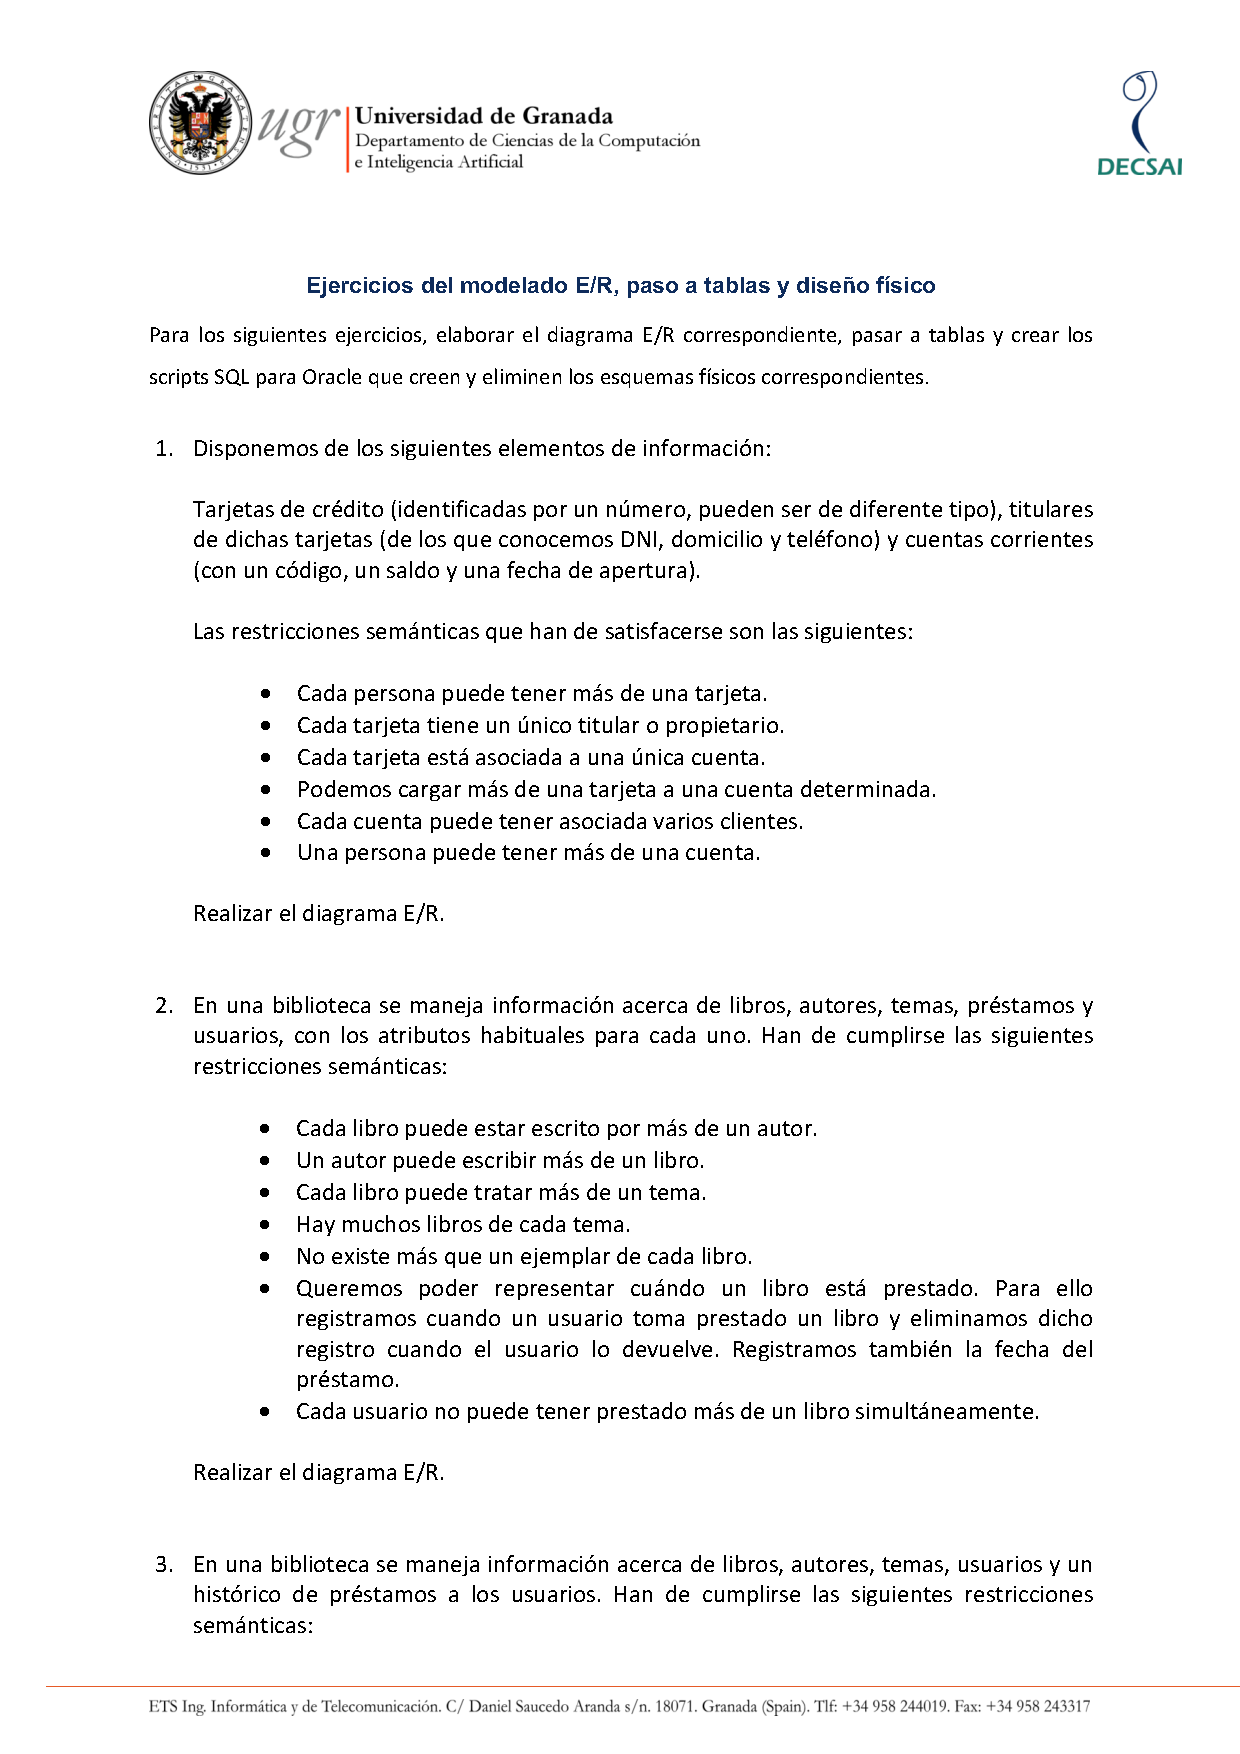
\includepdf[pages=-]{Capitulos/RelacionS1S2-SinEditar}%\includepdf[pages=-,pagecommand={\thispagestyle{fancy}}]{Capitulos/Ejercicios_FBD_S1.pdf}



% \begin{center}
%     \begin{tikzpicture}[
%         entity/.style={rectangle, draw, minimum width=3cm, minimum height=1cm},
%         relationship/.style={diamond, draw, minimum width=2cm, minimum height=1cm},
%         attribute/.style={ellipse, draw},
%         line/.style={draw, -latex},
%         singleline/.style={draw, -},
%         doubleline/.style={draw, double distance=2pt, -}
%     ]
%         % Entidades
%         \node[entity] (libro) {Libro};
%         \node[entity, right=4cm of libro] (autor) {Autor};
%         \node[entity, below=4cm of libro] (tema) {Tema};
%         \node[entity, below=4cm of autor] (usuario) {Usuario};

%         % Relaciones
%         \node[relationship, above right=1cm and 1cm of libro] (escribe) {Escribe};
%         \node[relationship, below=2cm of libro] (trata) {Trata de};
%         \node[relationship, below=2cm of escribe] (prestamo) {Préstamo};

%         % Atributos
%         \node[attribute, above left=1cm and 1cm of libro] (atributos_libro) {ISBN, Título};
%         \node[attribute, below left=1cm and 1cm of autor] (dni_autor) {DNI};
%         \node[attribute, below right=1cm and 1cm of autor] (domicilio_autor) {Domicilio};
%         \node[attribute, below left=1cm and 1cm of usuario] (dni_usuario) {DNI};
%         \node[attribute, below right=1cm and 1cm of usuario] (domicilio_usuario) {Domicilio};
%         \node[attribute, below=1cm of tema] (nombre_tema) {Nombre};

%         % Conexiones
%         \draw[doubleline] (libro) -- (escribe);
%         \draw[line] (escribe) -- (autor);
%         \draw[line] (libro) -- (trata);
%         \draw[line] (trata) -- (tema);
%         \draw[line] (libro) -- (prestamo);
%         \draw[line] (prestamo) -- (usuario);

%         \draw[line] (libro) -- (atributos_libro);
%         \draw[line] (autor) -- (dni_autor);
%         \draw[line] (autor) -- (domicilio_autor);
%         \draw[line] (usuario) -- (dni_usuario);
%         \draw[line] (usuario) -- (domicilio_usuario);
%         \draw[line] (tema) -- (nombre_tema);
%     \end{tikzpicture}
% \end{center}

\subsection{Ejercicio 1}
\begin{figure}[H]
    \begin{center}
        \begin{tikzpicture}[
            entity/.style={rectangle, draw, minimum width=3cm, minimum height=1cm},
            relationship/.style={diamond, draw, minimum width=2cm, minimum height=1cm},
            attribute/.style={ellipse, draw},
            line/.style={draw, -latex},
            singleline/.style={draw, -},
            doubleline/.style={draw, double distance=2pt, -},
        ]
            % Entidades
            \node[entity] (tarjeta) {Tarjeta};
            \node[entity, right=4cm of tarjeta] (cc) {C.C};
            \node[entity, below=4cm of tarjeta] (persona) {Persona};

            % Relaciones
            \node[relationship, above right=1cm and 1cm of tarjeta] (asociada) {Asociada};
            \node[relationship, below right=1cm and 1cm of cc] (vinculada) {Vinculada};
            \node[relationship, below left=1cm and 1cm of tarjeta] (titular) {Titular};

            % Atributos
            \node[attribute, above left=1cm and 1cm of tarjeta] (num_tarjeta) {\textbf{Nº}};
            \node[attribute, left=1cm of tarjeta] (tipo_tarjeta) {Tipo};
            \node[attribute, above right=1cm and 1cm of cc] (codigo_cc) {\b{Código}};
            \node[attribute, right=1cm of cc] (saldo_cc) {Saldo};
            \node[attribute, below left=1cm and 0.3cm of cc] (fecha_apertura_cc) {Fecha Apertura};
            \node[attribute, below left=1cm and 1cm of persona] (dni_persona) {\b{DNI}};
            \node[attribute, below=1cm of persona] (domicilio_persona) {Domicilio};
            \node[attribute, below right=1cm and 1cm of persona] (telefono_persona) {Teléfono};

            % Conexiones
            \draw[doubleline] (tarjeta) -- (asociada);
            \draw[line] (asociada) -- (cc);
            \draw[singleline] (cc) -- (vinculada);
            \draw[singleline] (vinculada) -- (persona);
            \draw[doubleline] (tarjeta) -- (titular);
            \draw[line] (titular) -- (persona);

            \draw[line, -*] (tarjeta) -- (num_tarjeta);  % Línea con círculo relleno al final
            \draw[line, -o] (tarjeta) -- (tipo_tarjeta); % Línea con círculo vacío al final
            \draw[line, -*] (cc) -- (codigo_cc);
            \draw[line, -o] (cc) -- (saldo_cc);
            \draw[line, -o] (cc) -- (fecha_apertura_cc);
            \draw[line, -*] (persona) -- (dni_persona);
            \draw[line, -o] (persona) -- (domicilio_persona);
            \draw[line,-o] (persona) -- (telefono_persona);
        \end{tikzpicture}
    \end{center}
    \caption{Diagrama Entidad-Relación del Ejercicio 1}
\end{figure}
\newpage
\foreach \n in {8,9,10,11,12,13,14,15,16,17,18,19,20,21,22,23,24,25,26} { 
    \begin{figure}[H]
        \centering
        \fbox{\includegraphics[width=\textwidth,height=\textheight,keepaspectratio]{Capitulos/Images_T1/EjerciciosP\n.png}}
        \caption{Relación de Ejercicios formato libreta página \n.}
        %\label{fig:ejercicio\n}
    \end{figure}
    \clearpage % Salto de página después de cada imagen
}



%\includepdf[pages=-,pagecommand={\thispagestyle{fancy}}]{Capitulos/Ejercicios_FBD_S1.pdf}



\newpage
% Referencias
\begin{thebibliography}{99}
\bibitem{Referencia1}
Ismael Sallami Moreno, \textbf{Estudiante del Doble Grado en Ingeniería Informática + ADE}, Universidad de Granada, 2025.
% \bibitem{Referencia2}
% Autor(es), \emph{Título del libro}, Editorial, año.

% \bibitem{Referencia3}
% Autor(es), \emph{Título del documento}, Nombre de la Conferencia, páginas, año.
\end{thebibliography}

\end{document}
